\documentclass[journal,12pt,twocolumn]{IEEEtran}

\usepackage{setspace}
\usepackage{gensymb}

\singlespacing


\usepackage[cmex10]{amsmath}

\usepackage{amsthm}

\usepackage{mathrsfs}
\usepackage{txfonts}
\usepackage{stfloats}
\usepackage{bm}
\usepackage{cite}
\usepackage{cases}
\usepackage{subfig}

\usepackage{longtable}
\usepackage{multirow}

\usepackage{enumitem}
\usepackage{mathtools}
\usepackage{steinmetz}
\usepackage{tikz}
\usepackage{circuitikz}
\usepackage{verbatim}
\usepackage{tfrupee}
\usepackage[breaklinks=true]{hyperref}
\usepackage{graphicx}
\usepackage{tkz-euclide}

\usetikzlibrary{calc,math}
\usepackage{listings}
    \usepackage{color}                                            %%
    \usepackage{array}                                            %%
    \usepackage{longtable}                                        %%
    \usepackage{calc}                                             %%
    \usepackage{multirow}                                         %%
    \usepackage{hhline}                                           %%
    \usepackage{ifthen}                                           %%
    \usepackage{lscape}     
\usepackage{multicol}
\usepackage{chngcntr}

\DeclareMathOperator*{\Res}{Res}

\renewcommand\thesection{\arabic{section}}
\renewcommand\thesubsection{\thesection.\arabic{subsection}}
\renewcommand\thesubsubsection{\thesubsection.\arabic{subsubsection}}

\renewcommand\thesectiondis{\arabic{section}}
\renewcommand\thesubsectiondis{\thesectiondis.\arabic{subsection}}
\renewcommand\thesubsubsectiondis{\thesubsectiondis.\arabic{subsubsection}}


\hyphenation{op-tical net-works semi-conduc-tor}
\def\inputGnumericTable{}                                 %%

\lstset{
%language=C,
frame=single, 
breaklines=true,
columns=fullflexible
}
\begin{document}


\newtheorem{theorem}{Theorem}[section]
\newtheorem{problem}{Problem}
\newtheorem{proposition}{Proposition}[section]
\newtheorem{lemma}{Lemma}[section]
\newtheorem{corollary}[theorem]{Corollary}
\newtheorem{example}{Example}[section]
\newtheorem{definition}[problem]{Definition}

\newcommand{\BEQA}{\begin{eqnarray}}
\newcommand{\EEQA}{\end{eqnarray}}
\newcommand{\define}{\stackrel{\triangle}{=}}
\bibliographystyle{IEEEtran}

\providecommand{\mbf}{\mathbf}
\providecommand{\pr}[1]{\ensuremath{\Pr\left(#1\right)}}
\providecommand{\qfunc}[1]{\ensuremath{Q\left(#1\right)}}
\providecommand{\sbrak}[1]{\ensuremath{{}\left[#1\right]}}
\providecommand{\lsbrak}[1]{\ensuremath{{}\left[#1\right.}}
\providecommand{\rsbrak}[1]{\ensuremath{{}\left.#1\right]}}
\providecommand{\brak}[1]{\ensuremath{\left(#1\right)}}
\providecommand{\lbrak}[1]{\ensuremath{\left(#1\right.}}
\providecommand{\rbrak}[1]{\ensuremath{\left.#1\right)}}
\providecommand{\cbrak}[1]{\ensuremath{\left\{#1\right\}}}
\providecommand{\lcbrak}[1]{\ensuremath{\left\{#1\right.}}
\providecommand{\rcbrak}[1]{\ensuremath{\left.#1\right\}}}
\theoremstyle{remark}
\newtheorem{rem}{Remark}
\newcommand{\sgn}{\mathop{\mathrm{sgn}}}
\providecommand{\abs}[1]{\left\vert#1\right\vert}
\providecommand{\res}[1]{\Res\displaylimits_{#1}} 
\providecommand{\norm}[1]{\left\lVert#1\right\rVert}
%\providecommand{\norm}[1]{\lVert#1\rVert}
\providecommand{\mtx}[1]{\mathbf{#1}}
\providecommand{\mean}[1]{E\left[ #1 \right]}
\providecommand{\fourier}{\overset{\mathcal{F}}{ \rightleftharpoons}}
%\providecommand{\hilbert}{\overset{\mathcal{H}}{ \rightleftharpoons}}
\providecommand{\system}{\overset{\mathcal{H}}{ \longleftrightarrow}}
	%\newcommand{\solution}[2]{\textbf{Solution:}{#1}}
\newcommand{\solution}{\noindent \textbf{Solution: }}
\newcommand{\cosec}{\,\text{cosec}\,}
\providecommand{\dec}[2]{\ensuremath{\overset{#1}{\underset{#2}{\gtrless}}}}
\newcommand{\myvec}[1]{\ensuremath{\begin{pmatrix}#1\end{pmatrix}}}
\newcommand{\mydet}[1]{\ensuremath{\begin{vmatrix}#1\end{vmatrix}}}
\numberwithin{equation}{subsection}

\makeatletter
\@addtoreset{figure}{problem}
\makeatother
\let\StandardTheFigure\thefigure
\let\vec\mathbf

\renewcommand{\thefigure}{\theproblem}

\def\putbox#1#2#3{\makebox[0in][l]{\makebox[#1][l]{}\raisebox{\baselineskip}[0in][0in]{\raisebox{#2}[0in][0in]{#3}}}}
     \def\rightbox#1{\makebox[0in][r]{#1}}
     \def\centbox#1{\makebox[0in]{#1}}
     \def\topbox#1{\raisebox{-\baselineskip}[0in][0in]{#1}}
     \def\midbox#1{\raisebox{-0.5\baselineskip}[0in][0in]{#1}}
\vspace{3cm}
\title{Assignment 3}
\author{Sachinkumar Dubey - EE20MTECH11009}

\maketitle
\newpage
\bigskip
\renewcommand{\thefigure}{\theenumi}
\renewcommand{\thetable}{\theenumi}
Download all python codes from 
\begin{lstlisting}
https://github.com/sachinomdubey/Matrix-theory/Assignment3/codes
\end{lstlisting}
%
and latex-tikz codes from 
%
\begin{lstlisting}
https://github.com/sachinomdubey/Matrix-theory/Assignment3
\end{lstlisting}
\subsection{Problem}
(Section 3.10) 60. Solve the system of linear equations using matrix method.
\begin{align}
    4x-3y=3 \\
    3x-5y=7
\end{align}
\subsection{Explanation}
The solution of linear equations can be obtained using matrix method as follow:
\begin{enumerate}
\item Write both the equations in matrix form.
\begin{align}
    \myvec{a & b}\vec{x}=c
\end{align}
    \item Form the Augmented matrix $(A|B)$.
    \item Reduce the augmented matrix to row echelon form.
    \item If $Rank(A)=Rank(A|B)$, then the system is said to be consistent. Further, there exist a unique solution if $Rank(A)=n$ (number of unknown) or infinite number of solutions if $Rank(A)<n$.
    \item If $Rank(A)\neq Rank(A|B)$, then the system is said to be inconsistent and no solution exists for the linear equations.
\end{enumerate}
\subsection{Solution}
Writing both euations in matrix form:
\begin{align}
    \myvec{4 & -3}\vec{x}=3\\
    \myvec{3 & -5}\vec{x}=7
\end{align}
Forming the augmented matrix and reducing the matrix to row echelon form:
\begin{align}
\myvec{4 & -3 & 3\\3 & -5 & 7}\\
\xleftrightarrow[]{R_1\leftarrow R_1/4}
\myvec{1 & -3/4 & 3/4\\3 & -5 & 7}\\
\xleftrightarrow[]{R_2\leftarrow R_2-3R_1}   
\myvec{1 & -3/4 & 3/4\\0 & -11/4 &19/4}\\
\xleftrightarrow[]{R_2\leftarrow R_2\times-4/11}
\myvec{1 & -3/4 & 3/4\\0 & 1 &-19/11}\\
\xleftrightarrow[]{R_1\leftarrow R_1+3/4\times R_2}
\myvec{1 & 0 & -6/11\\0 & 1 &-19/11} \label{eq7}
\end{align}
Here, $Rank(A)=Rank(A|B)$. Therefore, the system is consistent. Also, there exist a unique solution as $Rank(A)=n$ (number of unknown).\\ 
From equation \ref{eq7}, we get:
\begin{align}
    x=\frac{-6}{11}\\
    y=\frac{-19}{11}
\end{align}
Plotting the lines and the intersection point:
\begin{figure}[h!]
\centering
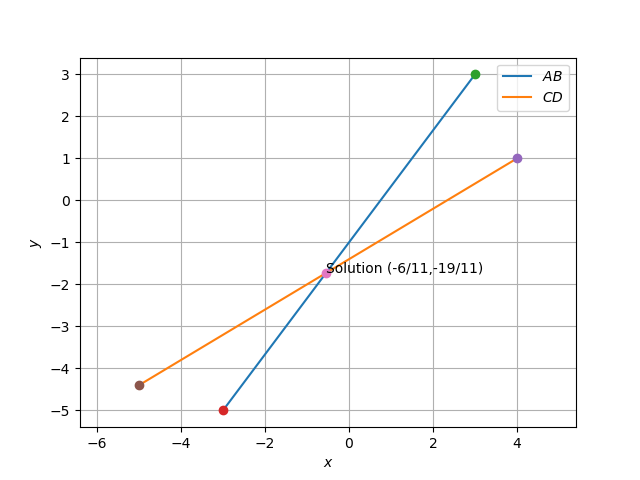
\includegraphics[width=8cm, height=7cm]{Figure_31}
\caption{Lines and their intersection denoting the solution}
\label{Fig4}
\end{figure}
\end{document}